\section{Exploratory Data Analysis}

\subsection{Statistics}
\label{chap:statistics}

\subsection{Dividing the Data}

Unlike classic machine learning processes, where data is split in three subsets, named train-, validation-, and test-set, here the data is split in four subsets.
The fourth data-set is used for backtesting the real trading strategy, and is therefore not part of the machine learning process but plays an important role in developing the final trading strategy.
In contrast, the test-set is only part of the machine learning process and is not used for evaluating or backtesting trading strategies.
This distinction was made so that the critical phases (testing machine learning models and testing trading strategies) cannot influence each other.

\begin{table}[H]
    \centering
    \begin{tabular}{ L{1.5cm} >{\centering\arraybackslash}m{4cm} >{\centering\arraybackslash}m{2cm} P{2.5cm} P{1.5cm} }
        \toprule
        Set & From & To & No.
        of Datapoints & \% of All Data
        \\
        \midrule
        \textbf{Complete} & \makecell{08/05/2022 \\ 10:00 UTC+2} & \makecell{06/17/2025 \\ 11:30 UTC+2} & $1,507,598$ & \\
        \addlinespace[0.8em]
        \textbf{Train} & \makecell{08/05/2022 \\ 10:00 UTC+2} & \makecell{04/30/2024 \\ 23:59 UTC+2} & $913,684$ & $60.6\%$ \\
        \addlinespace[0.8em]
        \textbf{Validation} & \makecell{05/01/2024 \\ 00:00 UTC+2} & \makecell{09/30/2024 \\ 23:59 UTC+2} & $220,320$ & $14.6\%$ \\
        \addlinespace[0.8em]
        \textbf{Test} & \makecell{10/01/2024 \\ 00:00 UTC+2} & \makecell{12/31/2024 \\ 23:59 UTC+2} & $132,482$ & $8.8\%$ \\
        \addlinespace[0.8em]
        \textbf{Backtest} & \makecell{01/01/2025 \\ 00:00 UTC+2} & \makecell{06/17/2025 \\ 11:30 UTC+2} & $241,111$ & $15.9\%$ \\
        \addlinespace[0.8em]
        \bottomrule
    \end{tabular}
    \caption{Data Split}
    \label{tbl:data-split}
\end{table}

\noindent
After the splitting, the four subsets have the following summaries:

\begin{table}[H]
    \centering
    \begin{tabular}{L{1.5cm}ccccc}
        \toprule
        & Open & High & Low & Close & Volume
        \\
        \midrule
        & Open & High & Low & Close & Volume
        \\
        \textbf{count} & 913684.0 & 913684.0 & 913684.0 & 913684.0 & 913684.0 \\
        \textbf{mean}  & 1933.4   & 1933.95  & 1932.85  & 1933.4   & 7.58     \\
        \textbf{std}   & 619.6    & 619.92   & 619.28   & 619.6    & 105.09   \\
        \textbf{min}   & 1074.35  & 1077.45  & 1064.05  & 1074.35  & 0.0      \\
        \textbf{25\%}  & 1578.44  & 1578.89  & 1577.99  & 1578.44  & 0.0      \\
        \textbf{50\%}  & 1801.52  & 1801.81  & 1801.13  & 1801.52  & 0.05     \\
        \textbf{75\%}  & 2083.4   & 2083.84  & 2083.05  & 2083.4   & 2.02     \\
        \textbf{max}   & 4098.5   & 4099.48  & 4096.35  & 4098.5   & 31350.65 \\
        \bottomrule
    \end{tabular}
    \caption{Train Data}
    \label{tbl:train-data}
\end{table}

\begin{table}[H]
    \centering
    \begin{tabular}{L{1.5cm}ccccc}
        \toprule
        & Open & High & Low & Close & Volume
        \\
        \midrule
        \textbf{count} & 220320.0 & 220320.0 & 220320.0 & 220320.0 & 220320.0 \\
        \textbf{mean}  & 3050.36  & 3051.3   & 3049.4   & 3050.36  & 2.89     \\
        \textbf{std}   & 473.4    & 473.45   & 473.34   & 473.4    & 21.45    \\
        \textbf{min}   & 2111.8   & 2160.4   & 2088.13  & 2111.8   & 0.0      \\
        \textbf{25\%}  & 2617.31  & 2618.04  & 2616.71  & 2617.31  & 0.0      \\
        \textbf{50\%}  & 3063.4   & 3064.31  & 3062.43  & 3063.4   & 0.12     \\
        \textbf{75\%}  & 3462.22  & 3463.29  & 3461.21  & 3462.22  & 1.32     \\
        \textbf{max}   & 3974.68  & 3976.96  & 3969.94  & 3974.68  & 4972.18  \\
        \bottomrule
    \end{tabular}
    \caption{Validation Data}
    \label{tbl:validation-data}
\end{table}

\begin{table}[H]
    \centering
    \begin{tabular}{L{1.5cm}ccccc}
        \toprule
        & Open & High & Low & Close & Volume
        \\
        \midrule
        \textbf{count} & 132482.0 & 132482.0 & 132482.0 & 132482.0 & 132482.0 \\
        \textbf{mean}  & 3093.93  & 3095.27  & 3092.58  & 3093.94  & 4.42     \\
        \textbf{std}   & 531.85   & 532.29   & 531.4    & 531.85   & 18.42    \\
        \textbf{min}   & 2309.01  & 2311.73  & 2307.73  & 2309.01  & 0.0      \\
        \textbf{25\%}  & 2541.8   & 2542.65  & 2540.94  & 2541.8   & 0.08     \\
        \textbf{50\%}  & 3143.69  & 3145.38  & 3142.02  & 3143.7   & 0.68     \\
        \textbf{75\%}  & 3487.9   & 3489.46  & 3486.33  & 3487.9   & 2.92     \\
        \textbf{max}   & 4107.28  & 4112.68  & 4102.6   & 4107.28  & 1341.05  \\
        \bottomrule
    \end{tabular}
    \caption{Test Data}
    \label{tbl:test-data}
\end{table}

\begin{table}[H]
    \centering
    \begin{tabular}{L{1.5cm}ccccc}
        \toprule
        & Open & High & Low & Close & Volume
        \\
        \midrule
        \textbf{count} & 241111.0 & 241111.0 & 241111.0 & 241111.0 & 241111.0 \\
        \textbf{mean}  & 2432.57  & 2433.77  & 2431.35  & 2432.57  & 7.0      \\
        \textbf{std}   & 574.72   & 574.95   & 574.49   & 574.72   & 32.11    \\
        \textbf{min}   & 1386.6   & 1395.8   & 1382.99  & 1386.6   & 0.0      \\
        \textbf{25\%}  & 1887.22  & 1888.28  & 1886.1   & 1887.22  & 0.18     \\
        \textbf{50\%}  & 2510.29  & 2511.4   & 2509.1   & 2510.29  & 1.26     \\
        \textbf{75\%}  & 2732.0   & 2733.21  & 2730.7   & 2732.0   & 4.94     \\
        \textbf{max}   & 3742.33  & 3745.13  & 3739.65  & 3742.33  & 2534.66  \\
        \bottomrule
    \end{tabular}
    \caption{Backtest Data}
    \label{tbl:backtest-data}
\end{table}

\subsection{Using Log-Returns}
\label{chap:log-returns}

In the summary statistics of the subsets (\autoref{tbl:train-data}, \autoref{tbl:validation-data}, \autoref{tbl:test-data}, \autoref{tbl:backtest-data}) it is noticeable that the mean values change over time.
This becomes also clear when visualizing the data (\autoref{fig:eth-data}).

\begin{figure}[H]
    \centering
    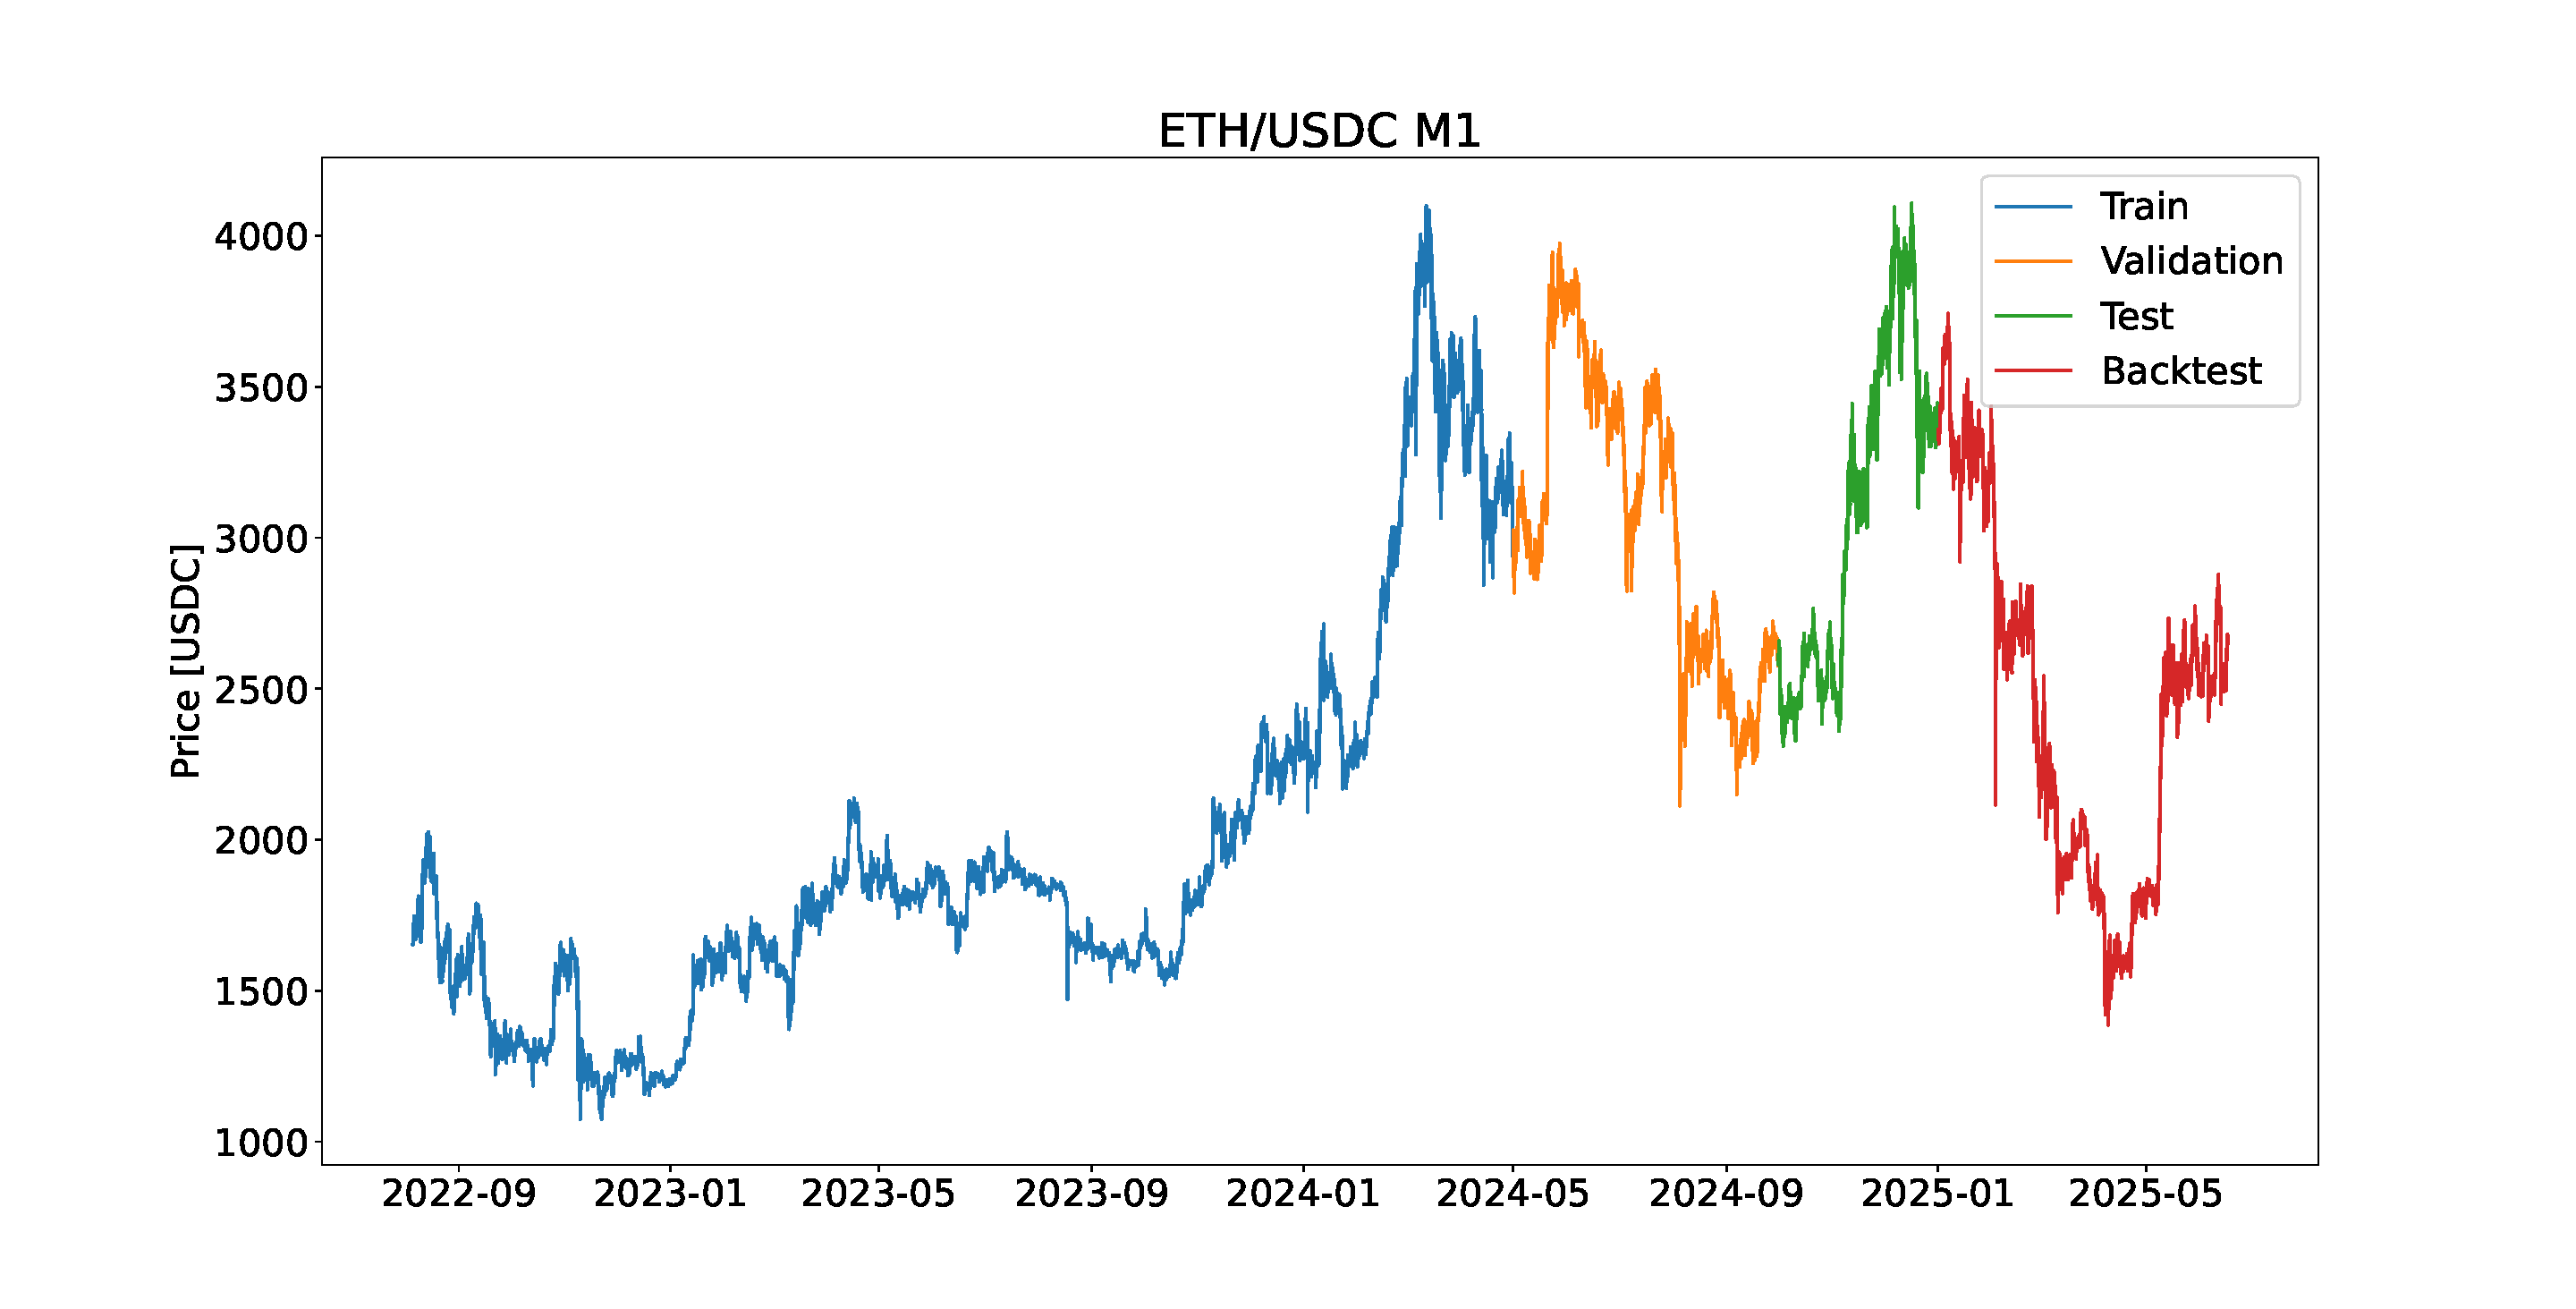
\includegraphics[width=\textwidth]{images/eda/ethusdc_price}
    \caption{Price Fluctuation of ETH in USDC}
    \label{fig:eth-data}
\end{figure}

\noindent
To avoid this data drift, the price is transformed to its logarithmic returns (also called log-returns).
These are calculated as follows:

\[
    LogReturn_t = ln(\frac{Price_t}{Price_{t-1}})
\]

\noindent
After the transformation, the means and standard deviations in the subsets are very similar, and the data does no longer drift over time.
\autoref{tbl:stat-log-returns} shows the means and standard deviations after the logarithmic return transformation.
Additionally, \autoref{fig:eth-log-data} shows visually that the data drift is eliminated.

\begin{table}[H]
    \centering
    \begin{tabular}{L{3cm}cc}
        \toprule
        Data Set            & Mean    & Standard Deviation \\
        \midrule
        \textbf{Train}      & 6.5E-7  & 8.7E-4             \\
        \textbf{Validation} & -6.1E-7 & 9.4E-4             \\
        \textbf{Test}       & 1.8E-6  & 9.4E-4             \\
        \textbf{Backtest}   & -9.5E-7 & 1.1E-3             \\
        \bottomrule
    \end{tabular}
    \caption{Statistics after Logarithmic Returns Transformation}
    \label{tbl:stat-log-returns}
\end{table}

\begin{figure}[H]
    \centering
    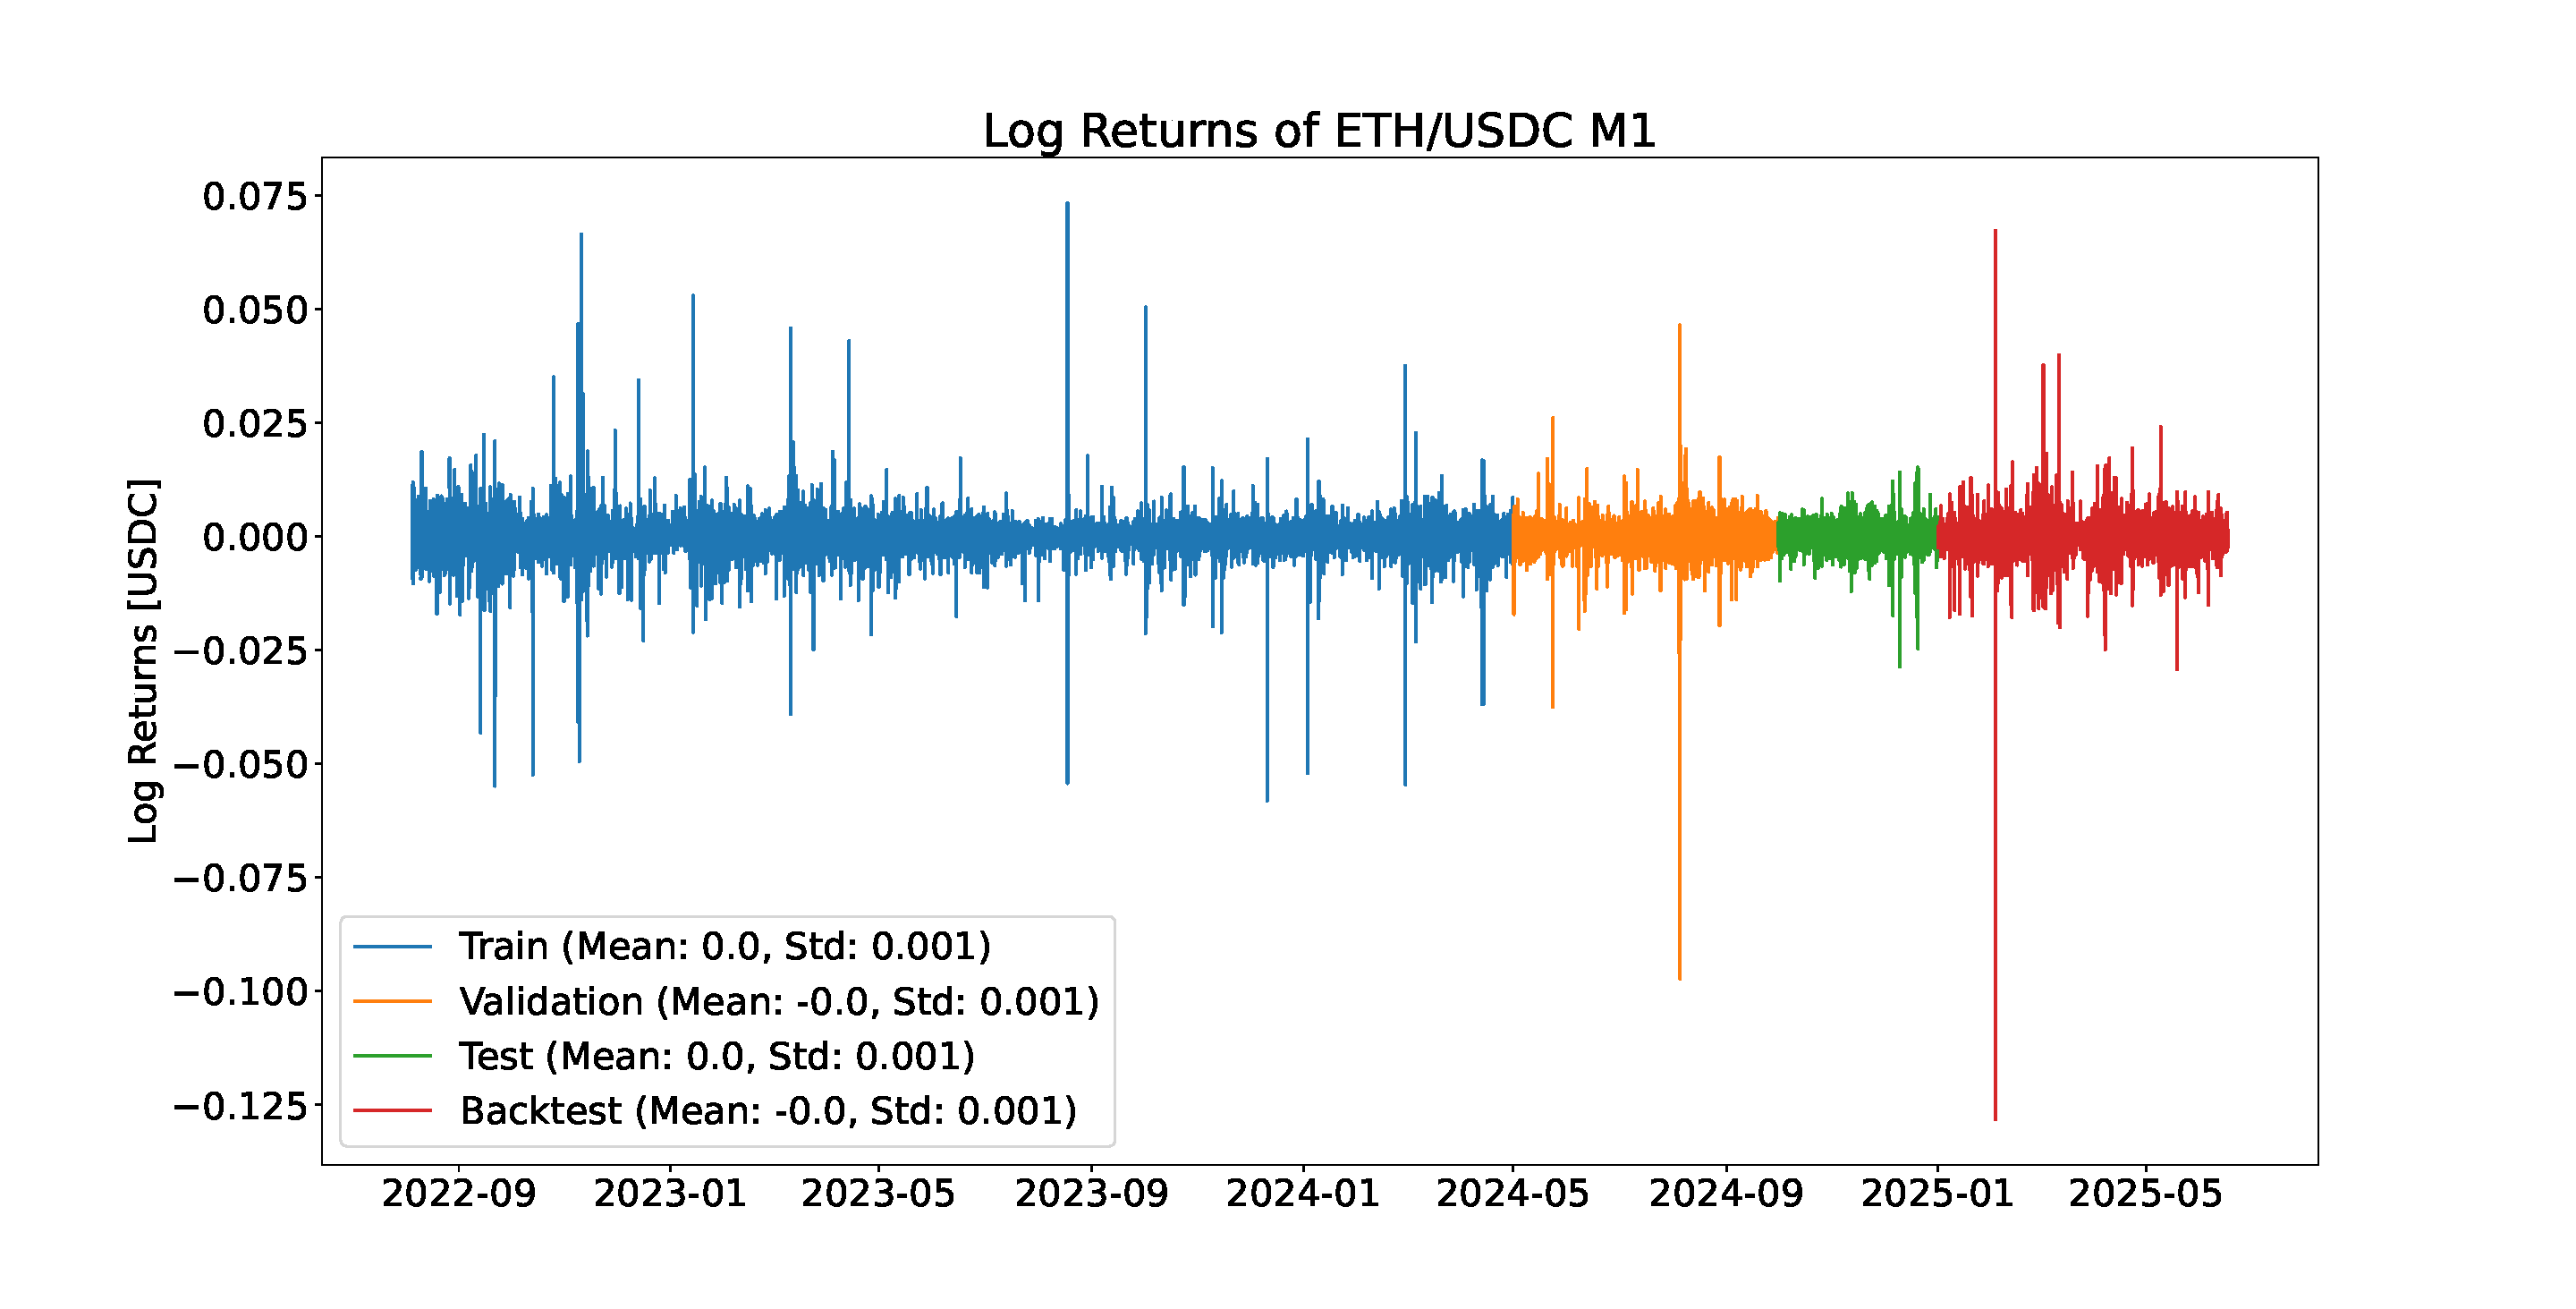
\includegraphics[width=\textwidth]{images/eda/log_returns_ethusdc}
    \caption{Log Returns of ETH in USDC}
    \label{fig:eth-log-data}
\end{figure}

\noindent
If an exact price is to be restored from the logarithmic returns, this can be done with the previous price using the following formula:

\[
    Price_t = Price_{t-1} * e^{LogReturn_t}
\]

\noindent
If a series of logarithmic returns is present, any price in the series can also be calculated using the following formula, where $Price_{0}$ is the price at the start of the series and $t$ is the distance to the start of the series:

\[
    Price_t = Price_0 * \prod_{i=0}^{t} e^{LogReturn_{i}} = Price_0 * e^{\sum_{i=0}^{t} LogReturn_i}
\]

\noindent
The transformation is applied to the open, high, low, and close prices, and the original prices are replaced by the logarithmic returns, so that all subsequent actions are carried out with the prices on the logarithmic returns.

\subsection{Additional Features}
\label{chap:additional-features}

To provide the machine learning models with more context about the price, additional features from different categories were added to the raw data.

\subsubsection{Trend Following Indicators}

In financial analysis trend following indicators play an essential role while modeling a predicting future price movements.
This occurs because markets move in trends that are repeatedly interrupted by outliers.
This results in a zigzag movement that nevertheless moves in one direction.
Trend-following indicators can be used to filter out these outliers \cite{investopia-trend-indicators}.

The exponential moving average (EMA) is one type of trend following indicator.
It is a variation of the classic simple moving average (SMA), placing more emphasis on newer prices.
It is often used by traders in length of 10-, 50-, and 200-period.
One limitation is that many trades believe that new data better reflects the current trend, where many others believe that overweighting recent prices creates a bias \cite{investopia-ema}.

%TODO: Bild von EMA und SMA im Vergleich -> EMA regiert schneller

Because the EMA reacts faster to price changes than the SMA, and the aim of this paper are short-term predictions, the EMA could provide more relevant context for the model.
The EMA was added in 5, 10, 20, 30, 50, and 200 period to the data.

Another Trend following indicator is the moving average convergence/divergence (MACD) which does not only help to identify price trends, but also helps to measure the trend momentum.
It shows the relationship between two exponential moving averages.
To calculate the MACD line, an EMA(12) is subtracted from an EMA(26).
Additionally, a signal line is calculated as an EMA(9) of the MACD line.

Although the MACD can signal possible reversals, it is also known for creating many false positives.
This often happens if the market moves sideways \cite{investopia-macd}.

\subsubsection{Volatility Indicators}

To measure volatility, there are other indicators and techniques to measure the volatility, in addition to those described in \autoref{chap:market-regime-categories}.

One indicator is the average true range (ATR) which decomposes the entire range of an asset price for a period.
It is calculated by determining the so-called true range (TR) for each candlestick - the maximum of: current high minus low; distance from the previous closing price up, and down.
The ATR is then the moving average of these TR values, usually over 14 periods.

The ATR has two main limitations.
The first is that an ATR value must always be set into comparison to previous ATR values, because one single value is not enough to tell if a trend is going to reverse.
The second limitation is that the ATR does not tell anything about the direction of the price \cite{investopia-atr}.
The ATR was added in 5, 7, 10, 14, and 18 periods to the data.

Another volatility indicator are Bollinger Bands, which consist of three lines.
The middle line is a SMA of the closing prices, the lower line is calculated by subtracting a certain number of standard deviations from the middle line, and the upper line is calculated by adding a certain number of standard deviations to the middle line.
Usually the double of the standard deviation is added, and subtracted from the middle line.

The higher the volatility of the market is in the last closing prices, the wider the band gets.
If the price of the market rises near the upper band, traders see the market as overbought.
Similarly, if the market falls near the lower band, the market could be oversold.
This allows to generate possible entry and exit signals \cite{investopia-bb}.
The three Lines where added to the data with a 15, 20, and 25 period SMA.

\subsubsection{Momentum Indicators}

Momentum measures the strength and direction of a price movement over a certain period of time.
Momentum indicators are useful because they give insights into the strength of trending prices.
Therefore, they can indicate possible reversals in the trend direction \cite{investopia-momentum}.

A common momentum indicator is the relative strength index (RSI).
It measures the speed and magnitude of an asset price by comparing the average gains and losses of the asset, and can be used to detect overbought and oversold conditions.
The RSI ranges between zero and 100.
Usually an RSI over 70 indicates an overbought, and an RSI below 30 indicates an oversold market.
Commonly the default RSI period to compare the average gains, and losses is 14 \cite{investopia-rsi}.
The RSI was added in periods 7, 14, and 20 to the data.

To depict relative trend strength, a sophisticated momentum indicator was constructed that compares the log returns of two different time frames.
This feature allows the model to distinguish phases of accelerating price movements from stable or declining trends.
The use of logarithmic returns simultaneously achieves scale independence, and improved comparability, which is particularly advantageous for modeling financial market-related time series.
This indicator was added for time frames M2, M3, M6, M9, and M12.

\subsubsection{Price Transformation Indicators}

Apart from the mentioned indicators shifted logarithmic returns for the last six minutes have been added to provide additional context about the last price movements in a compact form.
This could help the models to recognize trend reversals, volatility changes or short-term patterns.

Lastly, the logarithmic returns of other time frames (M2, M3, M6, M9, and M12) have been added to the data providing another more stable trend context which helps to correctly classify short-term price movements.
This creates a balanced feature set that takes into account both rapid reactions and long-term patterns.

\subsection{Scaling the Data}

Scaling data is an important step in exploratory data analysis.
This is because, on the one hand, machine learning models perform better with scaled data \cite{data-scaling}, and, on the other hand, principal component analysis (\autoref{chap:pca}) is sensitive to unscaled data \cite{pca-scaling}.

The use of the scikit-learn \texttt{MinMaxScaler} \cite{min-max}, which scales data date in a fixed range of $[0; 1]$ is useful and widely used.
Neural networks, especially those with activation functions such as ReLU, which is introduced in \autoref{chap:nn} benefits greatly from inputs with a uniform range of values.
The scaling stabilizes the gradient flow, shortens training time and reduces vanishing gradients \cite{min-max-benefits}.

For these reasons, all features were scaled with the \texttt{MinMaxScaler} and are used exclusively in the scaled form in all steps related to machine learning.

\subsection{Principal Component Analysis}
\label{chap:pca}

The principal component analysis (PCA) is a process for dimensional reduction, by linearly transforming high dimensional datasets to a small number of uncorrelated principal components  (directions of the new coordinate system).
During the transformation, it can be specified how much variance in the data can be eliminated.
After a transformation using PCA, it is ensured that at least the specified variance is retained \cite{wikipedia-pca}.

Especially when processing numerous technical indicators or derived features in financial data, the high dimensionality can become problematic - a phenomenon known as the course of dimensionality.
This term describes the increasing challenges in modeling as the number of dimensions or features increases.
Data points become increasingly sparsely disturbed, computational costs increase, and many models lose their ability to generalize.
Applying PCA allows redundant or correlated information to be condensed, making the model more robust, faster, and easier to interpret.
At the same time, the risk of overfitting is reduced because the model focuses on the most important structures in the dataset \cite{wikipedia-curse-od-dimensionality}.

\autoref{fig:explained-variance} shows the cumulative explained variance for the 56 added features in \autoref{chap:additional-features} for each quantile market regime.
It shows that the cumulative variance increases rapidly at the beginning.
In this case, the reduction of the project to just 3 to 6 principal components already explains at least 80\% of the variance.
This means that the majority of the statistically relevant structures in the dataset are retained, even though the number of features has been massively reduced.
Even if 20\% of the variance is lost, the benefit outweighs this: The remaining principal components capture the statistical essence of the original feature space in a significantly more compact and robust form, which is particularly well-suited for machine learning.


\begin{figure}[H]
    \centering
    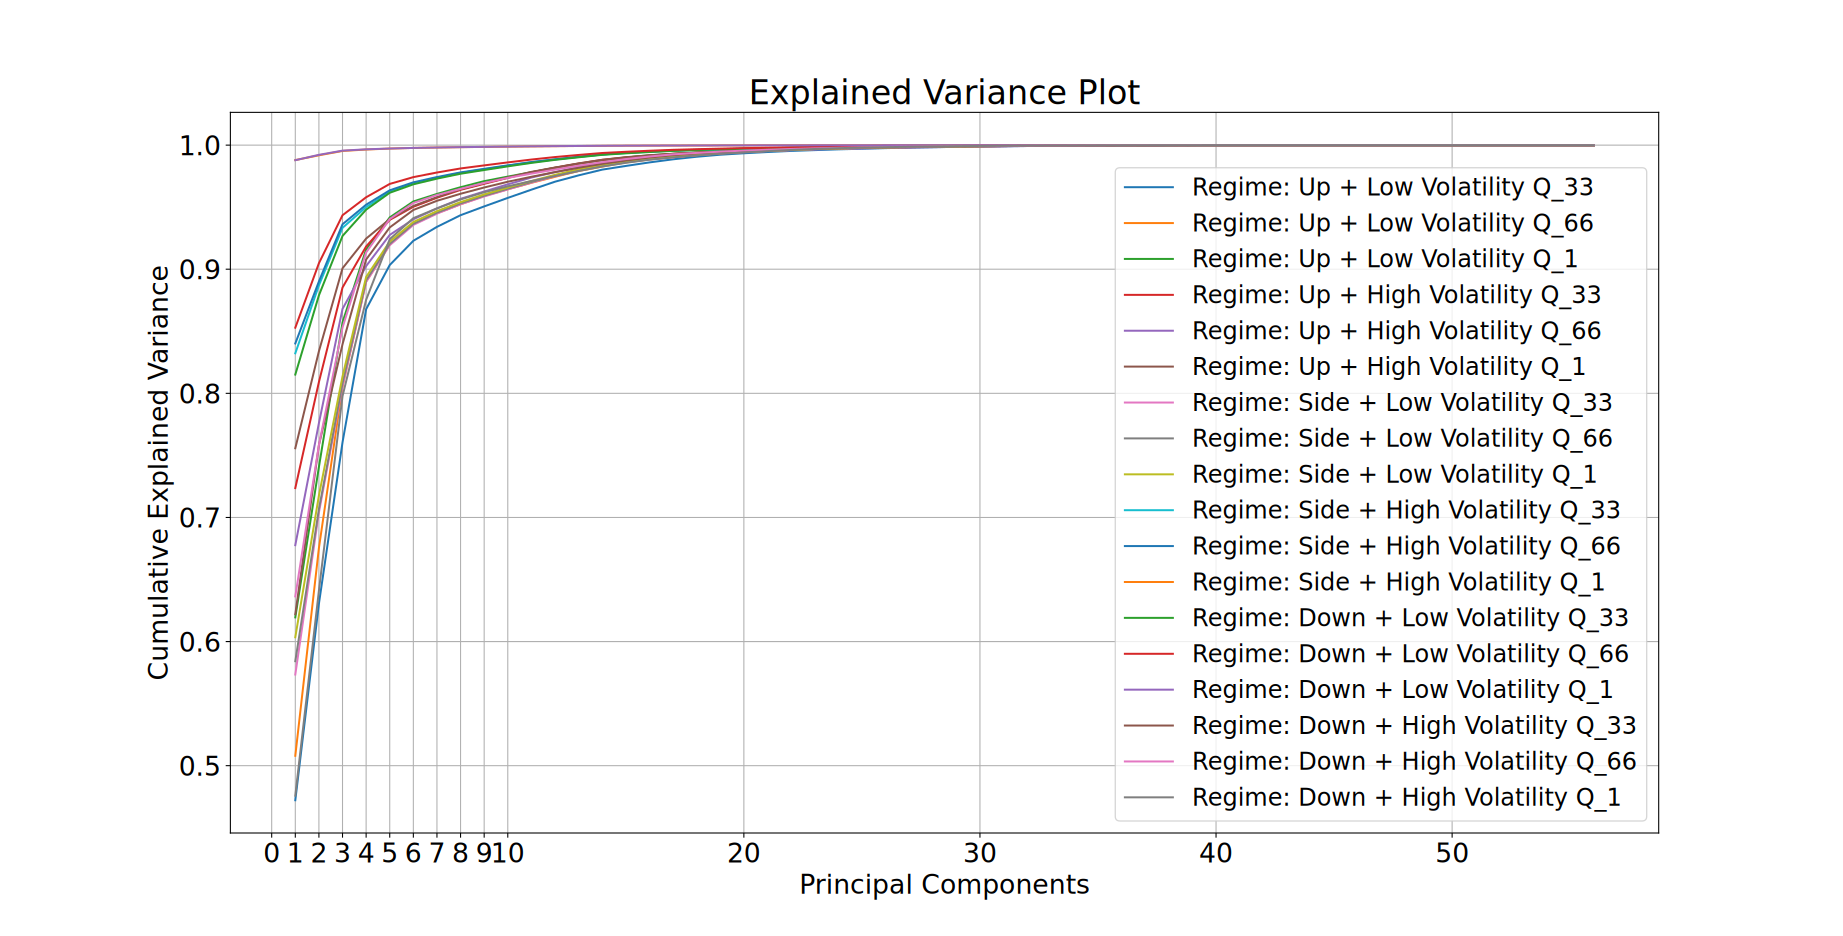
\includegraphics[width=\textwidth]{images/eda/explained_variance}
    \caption{Cumulative Explained Variance}
    \label{fig:explained-variance}
\end{figure}
